In the event of a batch update $\Delta^{t-} \cup \Delta^{t+}$ being relatively small compared to the total number of edges $|E|$, it is expected that only a small subset of vertices will undergo rank changes. To tackle this situation, our proposed approaches utilize an incremental process to identify affected vertices.

\begin{figure*}[hbtp]
  \centering
  \subfigure[Initial graph]{
    \label{fig:about-frontier-df1}
    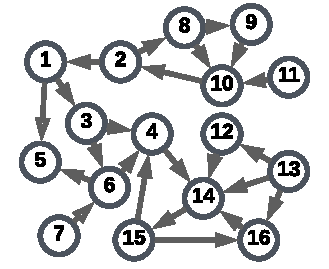
\includegraphics[width=0.23\linewidth]{out/about-frontier-11.pdf}
  }
  \subfigure[Marking initial affected vertices (DF)]{
    \label{fig:about-frontier-df2}
    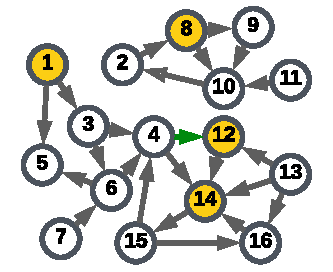
\includegraphics[width=0.23\linewidth]{out/about-frontier-32.pdf}
  }
  \subfigure[After first iteration (DF)]{
    \label{fig:about-frontier-df3}
    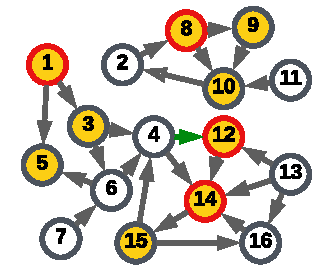
\includegraphics[width=0.23\linewidth]{out/about-frontier-33.pdf}
  }
  \subfigure[After second iteration (DF)]{
    \label{fig:about-frontier-df4}
    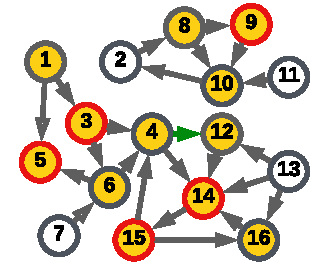
\includegraphics[width=0.23\linewidth]{out/about-frontier-34.pdf}
  } \\[2ex]
  \subfigure[Initial graph]{
    \label{fig:about-frontier-dfp1}
    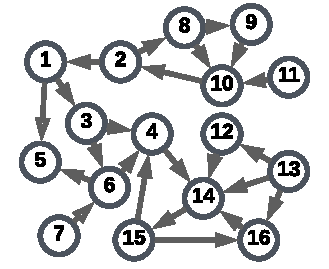
\includegraphics[width=0.23\linewidth]{out/about-frontier-11.pdf}
  }
  \subfigure[Marking initial affected vertices (DF-P)]{
    \label{fig:about-frontier-dfp2}
    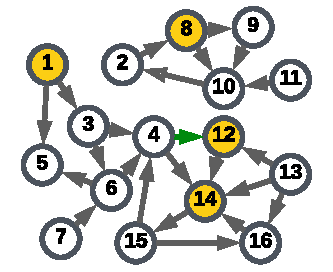
\includegraphics[width=0.23\linewidth]{out/about-frontier-32.pdf}
  }
  \subfigure[After first iteration (DF-P)]{
    \label{fig:about-frontier-dfp3}
    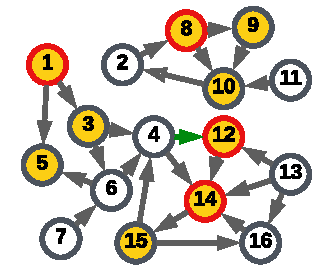
\includegraphics[width=0.23\linewidth]{out/about-frontier-33.pdf}
  }
  \subfigure[After second iteration (DF-P)]{
    \label{fig:about-frontier-dfp4}
    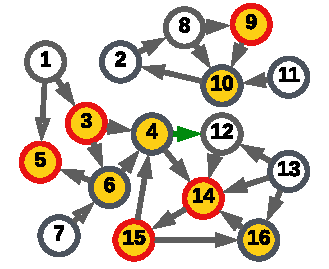
\includegraphics[width=0.23\linewidth]{out/about-frontier-44.pdf}
  } \\[2ex]
  \subfigure[Initial graph]{
    \label{fig:about-frontier-dt1}
    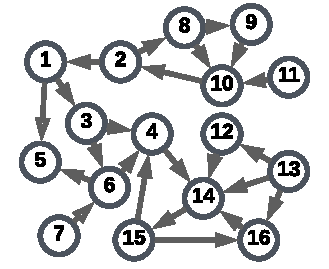
\includegraphics[width=0.23\linewidth]{out/about-frontier-11.pdf}
  }
  \subfigure[Marking affected vertices (DT)]{
    \label{fig:about-frontier-dt2}
    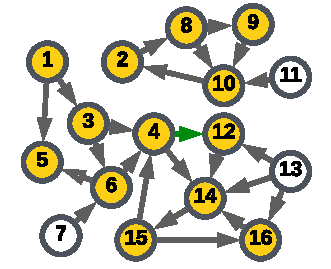
\includegraphics[width=0.23\linewidth]{out/about-frontier-22.pdf}
  }
  \subfigure[After first iteration (DT)]{
    \label{fig:about-frontier-dt3}
    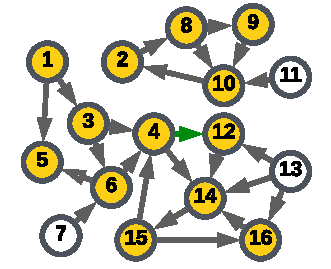
\includegraphics[width=0.23\linewidth]{out/about-frontier-22.pdf}
  }
  \subfigure[After second iteration (DT)]{
    \label{fig:about-frontier-dt4}
    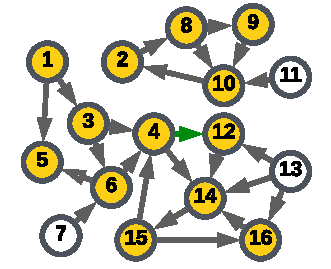
\includegraphics[width=0.23\linewidth]{out/about-frontier-22.pdf}
  } \\[-2ex]
  \caption{An example showcasing our improved \textit{Dynamic Frontier (DF)} and \textit{Dynamic Frontier with Pruning (DF-P)} approaches, in subfigures (a)-(d) and (e)-(h) respectively, in contrast to the \textit{Dynamic Traversal (DT)} approach, shown in subfigures (i)-(l).}
  \label{fig:about-frontier}
\end{figure*}

\ignore{An example showcasing our improved \textit{Dynamic Frontier (DF)} and \textit{Dynamic Frontier with Pruning (DF-P)} approaches. The initial graph has $16$ vertices and $23$ edges. The graph is updated with an edge insertion $(4, 12)$ and an edge deletion $(2, 1)$. Consequently, with DF and DF-P PageRank, the outgoing neighbors of vertices $2$ and $4$ (i.e., vertices $1$, $8$, $12$, and $14$) are marked as affected (shown with yellow fill). In the first iteration, when computing the ranks of these affected vertices, it is observed that the relative change in rank of vertices $1$, $8$, $12$, and $14$ exceeds the frontier tolerance $\tau_f$ (indicated with a red border). Therefore, their outgoing neighbors (i.e., vertices $3$, $5$, $9$, $10$, $14$, and $15$) are also marked as affected, with both DF and DF-P PageRank. In the second iteration, the relative rank change of vertices $3$, $5$, $9$, $14$, and $15$ surpasses the frontier tolerance $\tau_f$, resulting in their outgoing neighbors (i.e., vertices $4$, $6$, $10$, $15$, and $16$) being marked as affected. Additionally, with DF-P PageRank, vertices $1$, $8$, and $12$ are no longer marked as affected as their relative rank change falls below prune tolerance $\tau_p$. In the following iteration, the rankings of affected vertices are updated once more. If the rank change of each vertex falls within the iteration tolerance $\tau$, indicating convergence, the algorithm terminates. In contrast, the \textit{Dynamic Traversal (DT)} approach, marks all vertices reachable from $2$ and $4$ as affected. The ranks of this set of affected vertices are then updated in each iteration.}



\subsection{Our improved Dynamic Frontier approaches}
\label{sec:frontier}

We now explain our improved \textit{Dynamic Frontier (DF)} and \textit{Dynamic Frontier with Pruning (DF-P)} approaches. Consider a batch update with edge deletions $(u, v) \in \Delta^{t-}$ and insertions $(u, v) \in \Delta^{t+}$.


\subsubsection{Our improved Dynamic Frontier (DF) PageRank}

\paragraph{Initialization of ranks:}

Initially, we set the rank of each vertex to match the rank it had in the previous snapshot of the graph.

\paragraph{Initial marking of affected vertices:}

For every edge deletion/insertion $(u, v)$, mark the outgoing neighbors of vertex $u$ in both the previous snapshot $G^{t-1}$ and the current graph snapshot $G^t$, as affected.

\paragraph{Incremental expansion of the set of affected vertices upon change in rank of a given vertex:}

During the PageRank computation, if the rank of any affected vertex $v$ changes by a fraction exceeding the \textit{frontier tolerance} $\tau_f$, we designate its outgoing neighbors as affected. This step is taken because a modification in a vertex's rank is likely to impact the ranks of its outgoing neighbors. This process of marking vertices as affected continues in every iteration until the ranks have converged, as indicated by the iteration tolerance $\tau$.


\subsubsection{Our Dynamic Frontier with Pruning (DF-P) PageRank}

\paragraph{Initialization of ranks:}

We set the rank of each vertex to match the rank it had in the preceding snapshot of the graph.

\paragraph{Initial marking of affected vertices:}

For each edge deletion/insertion $(u, v)$, we mark the outgoing neighbors of vertex $u$ in both the previous $G^{t-1}$ and the current snapshot $G^t$ of the graph as affected.

\paragraph{Incremental expansion and contraction of the set of affected vertices upon change in rank of a given vertex:}

During PageRank computation, if the rank of any affected vertex $v$ changes in an iteration by a fraction greater than the \textit{frontier tolerance} $\tau_f$, we mark its outgoing neighbors as affected. Additionally, if the relative change in rank of a vertex remains below the \textit{prune tolerance} $\tau_p$, indicating potential convergence, the vertex is no longer marked as affected. However, if its rank has not converged, it may be re-marked as affected by one of its in-neighbors. This marking and unmarking process continues in every iteration, until the ranks have converged.

\paragraph{Computation of rank of each vertex}

As each vertex may be pruned (or unmarked as affected), and given that each vertex has a self-loop (as described in Sections \ref{sec:dataset} and \ref{sec:batch-generation}), we employ a closed-loop formula to calculate the rank of each vertex (Equation \ref{eq:pr-prune}). This formula accounts for the self-loop's presence, thereby reducing the need for recursive rank calculation due to the self-loop. The derivation of this formula is detailed in Section \ref{sec:pr-prune-derivation}.

\begin{flalign}
\label{eq:pr-prune}
  R[v] & = \frac{1}{1 - \alpha / |G.out(v)|} \left(\alpha K + \frac{1 - \alpha}{|V|}\right) && \\
    \text{where, } K & = \left(\sum_{u \in G.in(v)} \frac{R[u]}{|G.out(u)|}\right) - \frac{R[v]}{|G.out(v)|}
\end{flalign}


\subsubsection{A simple example}

Figure \ref{fig:about-frontier} illustrates an example of our improved Dynamic Frontier (DF) and Dynamic Frontier with Pruning (DF-P) PageRank. Initially, as depicted in Figures \ref{fig:about-frontier-df1} and \ref{fig:about-frontier-dfp1}, the graph comprises $16$ vertices and $23$ edges. Subsequently, Figures \ref{fig:about-frontier-df2} and \ref{fig:about-frontier-dfp2} show a batch update applied to the original graph, involving an edge insertion from vertex $4$ to $12$ and an edge deletion from vertex $2$ to $1$. Following the batch update, we proceed with the initial step of DF/DF-P PageRank, marking the outgoing neighbors of vertices $2$ and $4$ as affected, specifically vertices $1$, $8$, $12$, and $14$. These affected vertices are highlighted with a yellow fill. It may be noted that vertices $2$ and $4$ are not marked as affected. This is because changes in the out-degree of a vertex does not influence its PageRank score (see Equation \ref{eq:pr}). Subsequently, we initiate the first iteration of the PageRank algorithm.

During the first iteration (refer to Figures \ref{fig:about-frontier-df3} and \ref{fig:about-frontier-dfp3}), the ranks of affected vertices are updated. It is observed that the relative change in rank of vertices $1$, $8$, $12$, and $14$ exceeds the frontier tolerance $\tau_f$. Such vertices are indicated with a red border in the figures. In response to this, with both DF and DF-P PageRank, we incrementally mark the outgoing neighbors of vertices $1$, $8$, $12$, and $14$ as affected, specifically vertices $3$, $5$, $9$, $10$, $14$, and $15$

In the second iteration, shown in Figures \ref{fig:about-frontier-df4} and \ref{fig:about-frontier-dfp4}, updates are made to the ranks of affected vertices once again. Here, it is observed that the relative change in rank of vertices $3$, $5$, $9$, $14$, and $15$ exceeds the frontier tolerance $\tau_f$. Consequently, with DF/DF-P PageRank, we mark the outgoing neighbors of vertices $3$, $5$, $9$, $14$, and $15$ as affected, specifically vertices $4$, $6$, $10$, $15$, and $16$. Moreover, it is observed that the relative change in rank of vertices $1$, $8$, and $12$ remains below the prune tolerance $\tau_p$. As a result, with DF-P PageRank, these vertices are no longer marked as affected, as it is likely the ranks of such vertices have converged. This action effectively contracts the frontier of affected vertices. However, if the rank of such a vertex has not yet converged, it may be re-marked as affected by one of its in-neighbors.

In the next iteration, the ranks of affected vertices are updated once more. If the change in rank of each vertex remains within the iteration tolerance $\tau$ (we use $L\infty$-norm for convergence detection), the ranks of vertices have converged, and the algorithm terminates.

\paragraph{Contrasting with Dynamic Traversal (DT) PageRank}

Let us now contrast with DF and DF-P PageRank with Dynamic Traversal (DT) PageRank, shown in Figures \ref{fig:about-frontier-dt1}-\ref{fig:about-frontier-dt4}. Figure \ref{fig:about-frontier-dt2} show the same batch update applied to the original graph, as in Figures \ref{fig:about-frontier-df2} and \ref{fig:about-frontier-dfp2}. In response to this, DT PageRank marks all vertices reachable from $2$ and $4$ as affected, i.e., all vertices except $7$, $11$, and $13$. The ranks of this set of affected vertices are then updated in each iteration (ranks of unaffected vertices cannot change), until convergence.


\subsection{Determination of Frontier tolerance ($\tau_f$)}
\label{sec:frontier-tolerance}

We first need to determine a suitable approach for frontier expansion, and an associate frontier tolerance $\tau_f$ value that allows us to minimize processed vertices, while limiting error to that of ranks obtained with Static PageRank using the same iteration tolerance $\tau$. For this, we experiment with three approaches. These include marking neighbors of a vertex as affected, based on change in rank of the vertex $\Delta r$, change in its contribution factor $\Delta r/d$, or relative change in its rank $\Delta r/r$. Here, $\Delta r$ is the rank change, $d$ is the out-degree, and $r$ is the \texttt{max} of its previous and current rank values.

For $\Delta r$ and $\Delta r/d$, we adjust $\tau_f$ from $\tau$ to $\tau/10^5$; and for $\Delta r/r$, we adjust it from $0.1$ to $10^{-6}$. This is done on real-world dynamic graphs, shown in Table \ref{tab:dataset}, with batch updates of size $10^{-5}|E_T|$. Outgoing neighbors are marked affected if the respective measure exceeds $\tau_f$. Figure \ref{fig:adjust-frontier} shows the mean speedup (with respect to Static PageRank) and rank error (compared to ranks obtained with reference Static PageRank) with each approach for frontier expansion. Results indicate that the $\Delta r/r$ approach with a $\tau_f$ of $10^{-6}$ performs best, while yielding lower error than Static PageRank.

\begin{figure*}[!hbt]
  \centering
  \subfigure[Speedup with varying Frontier tolerance $\tau_f$]{
    \label{fig:adjust-frontier--speedup}
    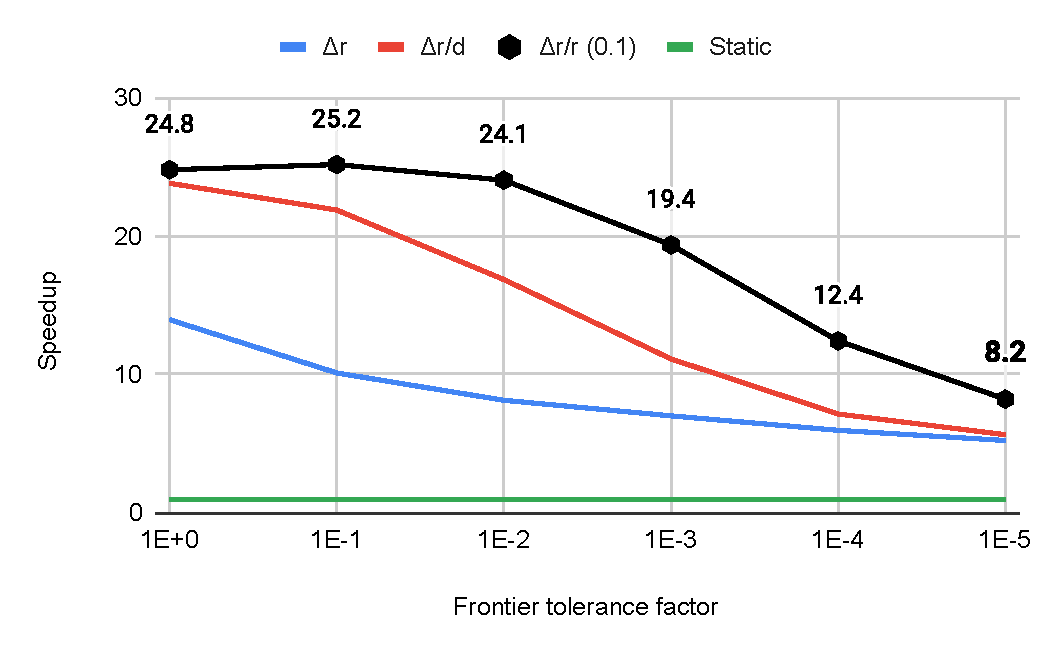
\includegraphics[width=0.48\linewidth]{out/adjust-frontier-speedup.pdf}
  }
  \subfigure[Error in ranks obtained with varying Frontier tolerance $\tau_f$]{
    \label{fig:adjust-frontier--error}
    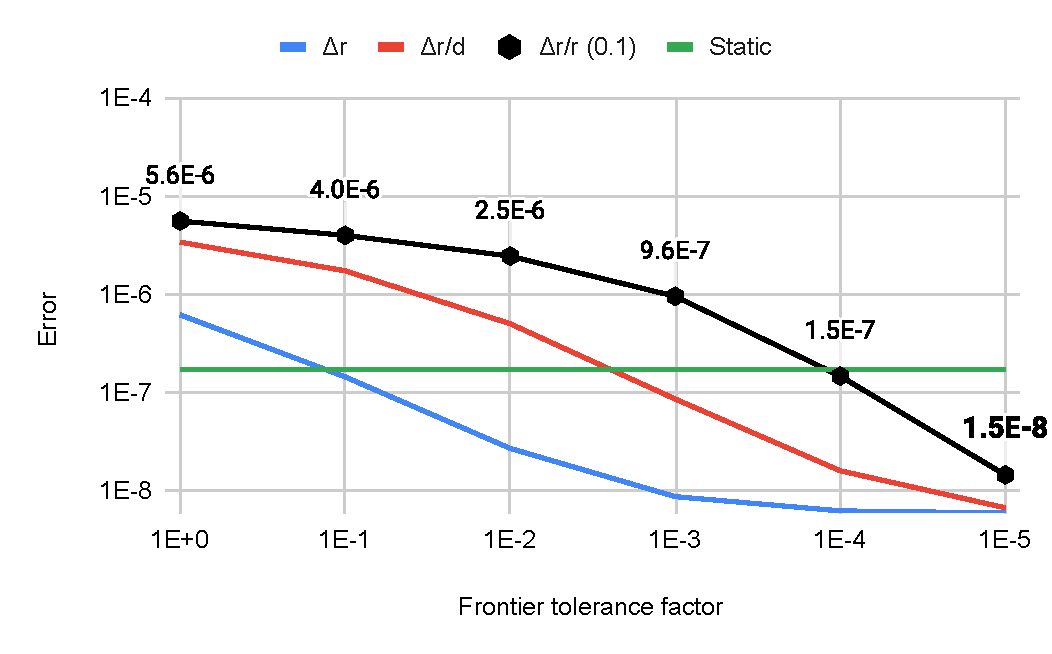
\includegraphics[width=0.48\linewidth]{out/adjust-frontier-error.pdf}
  } \\[-2ex]
  \caption{Average Speedup and Error in ranks obtained (with respect to ranks obtained with Reference Static PageRank) using \textit{Dynamic Frontier} approach, with frontier tolerance $\tau_f$ varying from $\tau$ to $\tau / 10^5$, on batch updates of size $10^{-7}|E|$ to $0.1|E|$. The figures indicate that increasing $\tau_f$ reduces runtime, but also increases the error. A Frontier tolerance $\tau_f$ of $\tau/10^4$ and $\tau/10^5$ obtain ranks with error lower than \textit{Static} PageRank, and are thus acceptable (we choose $\tau_f = \tau/10^5$ to be on the safe side).}
  \label{fig:adjust-frontier}
\end{figure*}

\begin{figure*}[!hbt]
  \centering
  \subfigure{
    \label{fig:adjust-prune--speedup}
    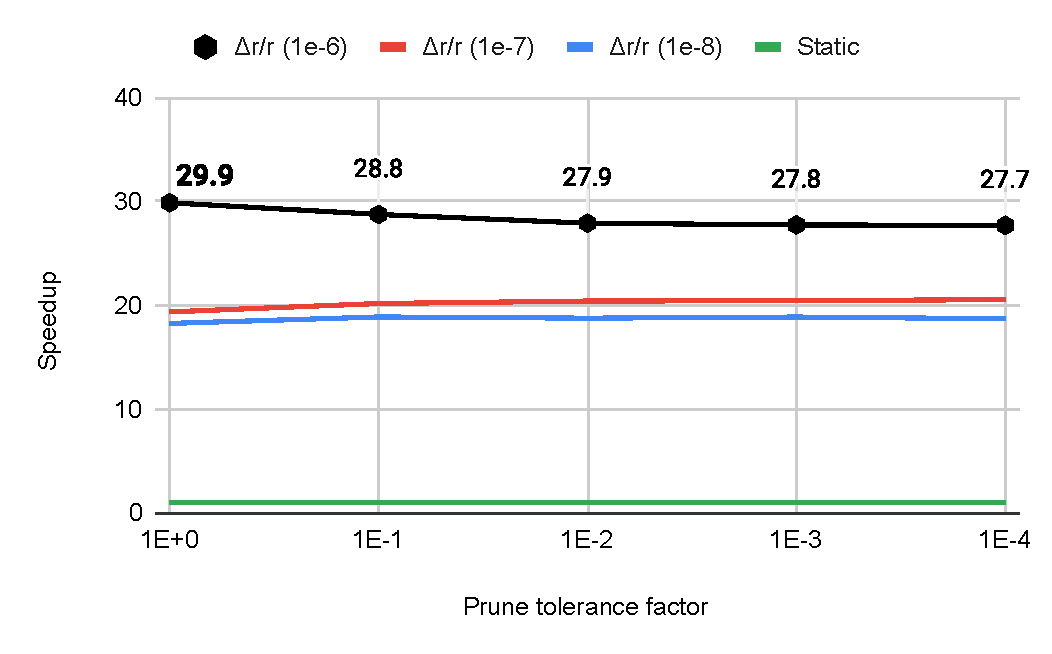
\includegraphics[width=0.48\linewidth]{out/adjust-prune-speedup.pdf}
  }
  \subfigure{
    \label{fig:adjust-prune--error}
    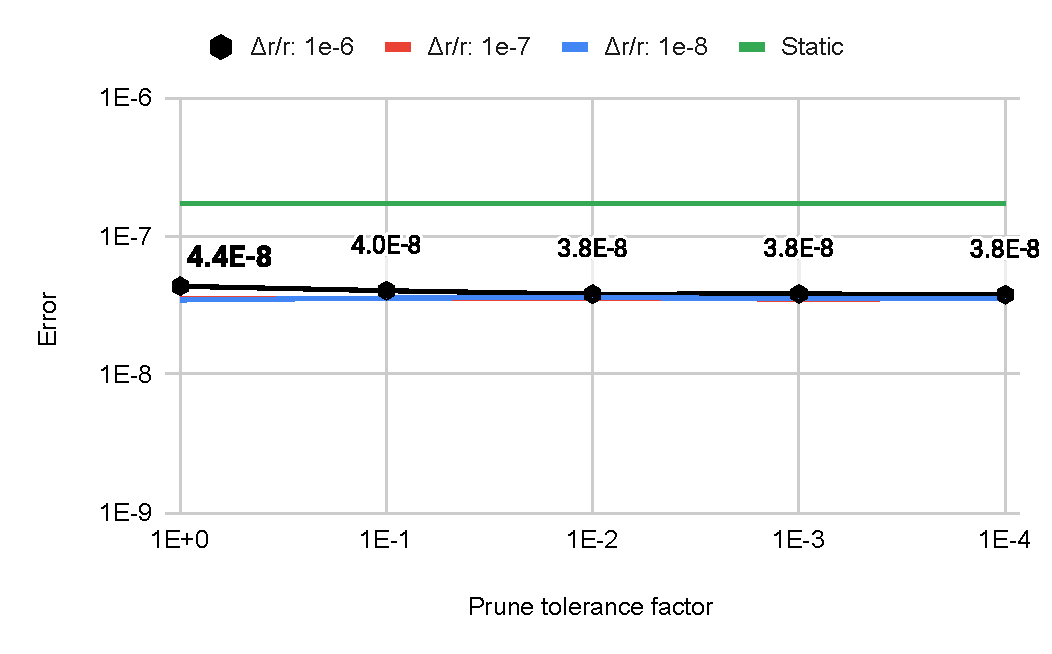
\includegraphics[width=0.48\linewidth]{out/adjust-prune-error.pdf}
  } \\[-2ex]
  \caption{Average Relative runtime with asynchronous implementations of \textit{Static}, \textit{Naive-dynamic}, \textit{Dynamic Traversal}, and \textit{Dynamic Frontier} approach compared to their respective synchronous implementations, on batch updates of size $10^{-7}|E|$ to $0.1|E|$ (right), and overall (left). The results indicate that asynchronous implementations are faster than synchronous ones, especially for smaller batch sizes. This is due to a somewhat faster convergence and the absence of copy overhead (for \textit{Dynamic Traversal} and \textit{Dynamic Frontier} approaches).}
  \label{fig:adjust-prune}
\end{figure*}

\begin{algorithm}[!hbt]
\caption{Our parallel Dynamic Frontier (DF) PageRank.}
\label{alg:frontier}
\begin{algorithmic}[1]
\Require{$G^{t-1}, G^t$: Previous, current input graph}
\Require{$\Delta^{t-}, \Delta^{t+}$: Edge deletions and insertions (input)}
\Require{$R^{t-1}, R$: Previous, current rank vector}
\Ensure{$\Delta r$: Change in rank of a vertex}
\Ensure{$\Delta R$: $L\infty$-norm between previous and current ranks}
\Ensure{$\tau, \tau_f, \tau_p$: Iteration, frontier, prune tolerance}
\Ensure{$\alpha$: Damping factor}

\Statex

\Function{dynamicFrontier}{$G^{t-1}, G^t, \Delta^{t-}, \Delta^{t+}, R^{t-1}$}
  \State $R \gets R^{t-1}$ \label{alg:frontier--initialize}
  \State $\rhd$ Mark initial affected
  \ForAll{$(u, v) \in \Delta^{t-} \cup \Delta^{t+} \textbf{in parallel}$} \label{alg:frontier--mark-begin}
    \ForAll{$v' \in (G^{t-1} \cup G^t).out(u)$}
    \State Mark $v'$ as affected
    \EndFor
  \EndFor \label{alg:frontier--mark-end}
  \ForAll{$i \in [0 .. MAX\_ITERATIONS)$} \label{alg:frontier--compute-begin}
    \State $\Delta R \gets 0$
    \ForAll{affected $v \in V^t$ \textbf{in parallel}}
      \State $r \gets (1 - \alpha)/|V^t|$
      \ForAll{$u \in G^t.in(v)$}
        \State $r \gets r + \alpha * R[u] / |G^t.out(u)|$
      \EndFor
      \State $\Delta r \gets |r - R[v]|$ \textbf{;} $\Delta R \gets \max(\Delta R, \Delta r)$
      \State $\rhd$ Prune $v$ if its relative rank change is small
      \If{$\Delta r / \max(r, R[v]) \leq \tau_p$}
        \State Mark $v$ as not affected
      \EndIf
      \State $\rhd$ Expand frontier if relative rank change is large
      \If{$\Delta r / \max(r, R[v]) > \tau_f$} \label{alg:frontier--remark-begin}
        \ForAll{$v' \in G^t.out(v)$}
          \State Mark $v'$ as affected
        \EndFor
      \EndIf \label{alg:frontier--remark-end}
      \State $\rhd$ Update rank of $v$
      \State $R[v] \gets r$
    \EndFor
    \State $\rhd$ Ranks converged?
    \If{$\Delta R \le \tau$} \textbf{break}
    \EndIf
  \EndFor \label{alg:frontier--compute-end}
  \State \ReturnInline{$R$} \label{alg:frontier--return}
\EndFunction
\end{algorithmic}
\end{algorithm}




%% Requires (parameters):
% G(V, E): a directed unweighted graph
% R: initial ranks (1/N for static)

%% Parameter values:
% MAX\_ITERATIONS = 500
% DAMPING\_FACTOR = 0.85
% TOLERANCE = 10^-10





\subsection{Determination of Prune tolerance ($\tau_p$)}
\label{sec:prune-tolerance}

We now embark on determining a suitable value for the prune tolerance $\tau_p$ to complement the optimal frontier expansion approach $\Delta r/r$, which employs a frontier tolerance $\tau_f$ of $10^{-6}$ as identified in Section \ref{sec:frontier-tolerance}. This entails adjusting $\tau_p$ from $\tau_f$ to $\tau_f/10^4$. Additionally, to err on the side of caution, we explore the effects of lower $\tau_f$ values, namely $10^{-7}$ and $10^{-8}$. These experiments are conducted on real-world graphs, employing batch updates of size $10^{-5}|E_T|$ as outlined earlier. A vertex is categorized as unaffected if its relative rank change $\Delta r/r$ falls within the designated $\tau_p$ range.

Figure \ref{fig:adjust-prune} presents the mean speedup, compared to Static PageRank, and the corresponding rank error observed when employing different $\tau_f$ values for frontier expansion. The rank error is measured with respect to reference Static PageRank, as discussed in Section \ref{sec:measurement}. Notably, the results highlight that the $\Delta r/r$ approach, particularly with a $\tau_f$ set to $10^{-6}$ and an accompanying $\tau_p$ of $\tau_f = 10^{-6}$, achieves superior performance by attaining lower rank error compared to Static PageRank.



\subsection{Our DF* PageRank implementation}

Algorithm \ref{alg:frontier} shows the pseudocode of our improved Dynamic Frontier (DF) and Dynamic Frontier with Pruning (DF-P) PageRank. Its takes as input the previous $G^{t-1}$ and current $G^t$ snapshot of the graph, edge deletions $\Delta^{t-}$ and insertions $\Delta^{t+}$ in the batch update, the previous rank vector $R^{t-1}$, and returns the updated ranks $R$.

The algorithm begins by initializing the current rank vector $R$ with the previous rank vector $R^{t-1}$ (line \ref{alg:frontier--initialize}), and marking the initially affected vertices based on edge deletions $\Delta^{t-}$ and insertions $\Delta^{t+}$ in parallel (lines \ref{alg:frontier--mark-begin}-\ref{alg:frontier--mark-end}). It then iteratively computes the rank $R[v]$ for each affected vertex $v$ (lines \ref{alg:frontier--compute-begin}-\ref{alg:frontier--compute-end}). This computation is performed in parallel, considering the incoming edges $G^t.in(v)$. Depending on whether DF or DF-P PageRank is selected, the corresponding formula for rank calculation is applied (lines \ref{alg:frontier--formula-begin}-\ref{alg:frontier--formula-end}). The algorithm then checks if the relative change in rank $\Delta r / \max(r, R[v])$ exceeds the frontier tolerance $\tau_f$, marking out-neighbor vertices as affected if so. Additionally, with DF-P PageRank, if the relative change in rank lies within the prune tolerance $\tau_p$, the vertex $v$ is marked as not affected. The iteration continues until either the maximum change in ranks $\Delta R$ falls below the iteration tolerance $\tau$, or the maximum number of iterations $MAX\_ITERATIONS$ is reached. Finally, the algorithm returns the final rank vector $R$ (line \ref{alg:frontier--return}).

In a push-based approach for PageRank computation, each thread calculates and sums the outgoing PageRank contribution of its vertex to its neighbors, necessitating atomic updates. In contrast, with a pull-based approach, each vertex's rank is updated through a single write by a thread \cite{verstraaten2015quantifying}. We find this to be more efficient and employ it for all implementations. Furthermore, we employ an asynchronous implementation of DF and DF-P PageRank, using a single rank vector, for potentially faster convergence and elimination of memory copies for unaffected vertices. This, based on our previous research \cite{sahu2024incrementally}, outperforms synchronous implementations, especially with smaller batch sizes. We also utilize asynchronous implementations for Naive-dynamic (ND) and Dynamic Traversal (DT) PageRank, but not for Static PageRank (async not faster).
